% Created 2025-09-30 Tue 13:56
% Intended LaTeX compiler: pdflatex
\documentclass[a4paper,12pt]{article}
\usepackage[utf8]{inputenc}
\usepackage[T1]{fontenc}
\usepackage{amsmath}
\usepackage{amssymb}
\usepackage{capt-of}
\usepackage{hyperref}
\usepackage{amsthm}
\usepackage{amssymb}
\usepackage{mathtools}
%\documentclass[12pt]{article}
\usepackage{geometry}

\usepackage{amsmath}
\usepackage{amssymb,amsfonts,textcomp}
\usepackage[T1]{fontenc}
\usepackage[utf8]{inputenc}
\usepackage{times} % Times New Roman font
\usepackage{setspace}
\usepackage[pdftex]{graphicx}

\usepackage{hyperref}

% Set line spacing to 1.5
\setstretch{1.5}

\geometry{a4paper, portrait, margin=0.7in, nohead}

\usepackage{titlesec}
\titleformat{\section}[block]{\normalfont\large\bfseries}{\thesection}{1em}{}
\titleformat{\subsection}[block]{\normalfont\large\bfseries}{\thesubsection}{1em}{}

\makeatletter

\newcommand{\student}[1]{\author{#1}}

\newcommand{\group}[1]{\def\@group{#1}}

\newcommand{\prof}[1]{\def\@prof{#1}}
\newcommand{\profdep}[1]{\def\@profdep{#1}}

\newcommand{\labno}[1]{\def\@labno{#1}}

\newcommand{\labtopic}[1]{\title{#1}}

\labsubject{Cryptography}
\group{FAF--233}
\prof{Zaica, asist. univ.}
\profdep{sea, fcim utm}
\labno{1}

%% ox-latex features:
%   !announce-start, !guess-pollyglossia, !guess-babel, !guess-inputenc,
%   engraved-code, caption, maths, image, !announce-end.

% Setup for code blocks [1/2]

\usepackage{fvextra}

\fvset{%
  commandchars=\\\{\},
  highlightcolor=white!95!black!80!blue,
  breaklines=true,
  breaksymbol=\color{white!60!black}\tiny\ensuremath{\hookrightarrow}}

% Make line numbers smaller and grey.
\renewcommand\theFancyVerbLine{\footnotesize\color{black!40!white}\arabic{FancyVerbLine}}

\usepackage{xcolor}

% In case engrave-faces-latex-gen-preamble has not been run.
\providecolor{EfD}{HTML}{f7f7f7}
\providecolor{EFD}{HTML}{28292e}

% Define a Code environment to prettily wrap the fontified code.
\usepackage[breakable,xparse]{tcolorbox}
\providecommand{\codefont}{\footnotesize}
\DeclareTColorBox[]{Code}{o}%
{colback=EfD!98!EFD, colframe=EfD!95!EFD,
  fontupper=\setlength{\fboxsep}{0pt}\codefont,
  colupper=EFD,
  IfNoValueTF={#1}%
  {boxsep=2pt, arc=2.5pt, outer arc=2.5pt,
    boxrule=0.5pt, left=2pt}%
  {boxsep=2.5pt, arc=0pt, outer arc=0pt,
    boxrule=0pt, leftrule=1.5pt, left=0.5pt},
  right=2pt, top=1pt, bottom=0.5pt,
  breakable}

% Support listings with captions
\usepackage{float}
\floatstyle{plain}
\newfloat{listing}{htbp}{lst}
\newcommand{\listingsname}{Listing}
\floatname{listing}{\listingsname}
\newcommand{\listoflistingsname}{List of Listings}
\providecommand{\listoflistings}{\listof{listing}{\listoflistingsname}}


% Setup for code blocks [2/2]: syntax highlighting colors

\newcommand\efstrut{\vrule height 2.1ex depth 0.8ex width 0pt}
\definecolor{EFD}{HTML}{000000}
\definecolor{EfD}{HTML}{ffffff}
\newcommand{\EFD}[1]{\textcolor{EFD}{#1}} % default
\definecolor{EFh}{HTML}{7f7f7f}
\newcommand{\EFh}[1]{\textcolor{EFh}{#1}} % shadow
\definecolor{EFsc}{HTML}{228b22}
\newcommand{\EFsc}[1]{\textcolor{EFsc}{\textbf{#1}}} % success
\definecolor{EFw}{HTML}{ff8e00}
\newcommand{\EFw}[1]{\textcolor{EFw}{\textbf{#1}}} % warning
\definecolor{EFe}{HTML}{ff0000}
\newcommand{\EFe}[1]{\textcolor{EFe}{\textbf{#1}}} % error
\definecolor{EFc}{HTML}{b22222}
\newcommand{\EFc}[1]{\textcolor{EFc}{#1}} % font-lock-comment-face
\definecolor{EFcd}{HTML}{b22222}
\newcommand{\EFcd}[1]{\textcolor{EFcd}{#1}} % font-lock-comment-delimiter-face
\definecolor{EFs}{HTML}{8b2252}
\newcommand{\EFs}[1]{\textcolor{EFs}{#1}} % font-lock-string-face
\definecolor{EFd}{HTML}{8b2252}
\newcommand{\EFd}[1]{\textcolor{EFd}{#1}} % font-lock-doc-face
\definecolor{EFm}{HTML}{008b8b}
\newcommand{\EFm}[1]{\textcolor{EFm}{#1}} % font-lock-doc-markup-face
\definecolor{EFk}{HTML}{9370db}
\newcommand{\EFk}[1]{\textcolor{EFk}{#1}} % font-lock-keyword-face
\definecolor{EFb}{HTML}{483d8b}
\newcommand{\EFb}[1]{\textcolor{EFb}{#1}} % font-lock-builtin-face
\definecolor{EFf}{HTML}{0000ff}
\newcommand{\EFf}[1]{\textcolor{EFf}{#1}} % font-lock-function-name-face
\definecolor{EFv}{HTML}{a0522d}
\newcommand{\EFv}[1]{\textcolor{EFv}{#1}} % font-lock-variable-name-face
\definecolor{EFt}{HTML}{228b22}
\newcommand{\EFt}[1]{\textcolor{EFt}{#1}} % font-lock-type-face
\definecolor{EFo}{HTML}{008b8b}
\newcommand{\EFo}[1]{\textcolor{EFo}{#1}} % font-lock-constant-face
\definecolor{EFwr}{HTML}{ff0000}
\newcommand{\EFwr}[1]{\textcolor{EFwr}{\textbf{#1}}} % font-lock-warning-face
\newcommand{\EFnc}[1]{#1} % font-lock-negation-char-face
\definecolor{EFpp}{HTML}{483d8b}
\newcommand{\EFpp}[1]{\textcolor{EFpp}{#1}} % font-lock-preprocessor-face
\newcommand{\EFrc}[1]{\textbf{#1}} % font-lock-regexp-grouping-construct
\newcommand{\EFrb}[1]{\textbf{#1}} % font-lock-regexp-grouping-backslash
\newcommand{\EFob}[1]{#1} % org-block
\definecolor{EFhn}{HTML}{008b8b}
\newcommand{\EFhn}[1]{\textcolor{EFhn}{#1}} % highlight-numbers-number
\definecolor{EFhq}{HTML}{9370db}
\newcommand{\EFhq}[1]{\textcolor{EFhq}{#1}} % highlight-quoted-quote
\definecolor{EFhs}{HTML}{008b8b}
\newcommand{\EFhs}[1]{\textcolor{EFhs}{#1}} % highlight-quoted-symbol
\definecolor{EFrda}{HTML}{707183}
\newcommand{\EFrda}[1]{\textcolor{EFrda}{#1}} % rainbow-delimiters-depth-1-face
\definecolor{EFrdb}{HTML}{7388d6}
\newcommand{\EFrdb}[1]{\textcolor{EFrdb}{#1}} % rainbow-delimiters-depth-2-face
\definecolor{EFrdc}{HTML}{909183}
\newcommand{\EFrdc}[1]{\textcolor{EFrdc}{#1}} % rainbow-delimiters-depth-3-face
\definecolor{EFrdd}{HTML}{709870}
\newcommand{\EFrdd}[1]{\textcolor{EFrdd}{#1}} % rainbow-delimiters-depth-4-face
\definecolor{EFrde}{HTML}{907373}
\newcommand{\EFrde}[1]{\textcolor{EFrde}{#1}} % rainbow-delimiters-depth-5-face
\definecolor{EFrdf}{HTML}{6276ba}
\newcommand{\EFrdf}[1]{\textcolor{EFrdf}{#1}} % rainbow-delimiters-depth-6-face
\definecolor{EFrdg}{HTML}{858580}
\newcommand{\EFrdg}[1]{\textcolor{EFrdg}{#1}} % rainbow-delimiters-depth-7-face
\definecolor{EFrdh}{HTML}{80a880}
\newcommand{\EFrdh}[1]{\textcolor{EFrdh}{#1}} % rainbow-delimiters-depth-8-face
\definecolor{EFrdi}{HTML}{887070}
\newcommand{\EFrdi}[1]{\textcolor{EFrdi}{#1}} % rainbow-delimiters-depth-9-face


\usepackage{capt-of}

\usepackage{amsmath}
\usepackage{amssymb}

\usepackage{graphicx}

%% end ox-latex features


\author{Andrei Chicu}
\date{\today}
\title{Caesar Cipher: Implementation \& Extension}
\hypersetup{
 pdfauthor={Andrei Chicu},
 pdftitle={Caesar Cipher: Implementation \& Extension},
 pdfkeywords={},
 pdfsubject={},
 pdfcreator={Emacs 30.2 (Org mode 9.8-pre)},
 pdflang={English}}
\begin{document}

\makeatletter
\begin{titlepage}
\centering


\includegraphics[height=2cm]{utm_logo.png}

\bfseries
\textsc{Ministry of Education and Research of Republic of Moldova} \\
\textsc{Technical University of Moldova} \\
\textsc{Faculty of Computers, Informatics and Microelectronics} \\
\textsc{Department of Software and Automation Engineering} \\
\mdseries

\vfill

\textsc{\Large \@labsubject} \\
\textsc{\large Laboratory work \#\@labno}\\[0.5cm]

\vspace{12pt}
\newcommand{\HRule}{\rule{\linewidth}{0.5mm}}
\HRule \\[0.2cm]
{ \LARGE \bfseries \@title }\\[0.4cm]
\HRule
\vfill

\begin{minipage}[t]{0.4\textwidth}
\begin{flushleft} \large
\emph{Author:} \\
\@author\\                        
std. gr. \@group
\end{flushleft}
\end{minipage}
~
\begin{minipage}[t]{0.4\textwidth}
\raggedleft \large
\emph{Verified:} \\
\@prof \\
Department of \textsc{\@profdep}
\end{minipage}\\[3cm]
\vfill

Chișinău, 2025
\end{titlepage}
\makeatother
\setcounter{page}{2}
\section{Introduction}
\label{sec:org6afa552}
GitHub repository: \url{https://github.com/andyp1xe1/crypto_labs}
\subsection{Objective}
\label{sec:org2501181}
The objective of this laboratory work is to implement the Caesar Cipher algorithm, covering both the standard fixed-shift version and an extended version that uses a keyword to permute the alphabet, significantly increasing the cipher's key space and cryptoresistance.
\subsection{Tasks}
\label{sec:org2732daa}
\begin{itemize}
\item Task 1.1: Standard Caesar Cipher (Single Key \(k_{1}\))
\item Task 1.2: Permutation Caesar Cipher (Two Keys \(k_{1}\) and \(k_{2}\))
\item Task 1.3: Cipher Verification (Exchange and Decrypt)
\end{itemize}
\subsection{Theoretical Background}
\label{sec:org42d0c6b}
The Caesar cipher is a substitution cipher where each letter in the plaintext is shifted by a fixed number of positions in the alphabet. The standard Caesar cipher uses the following formulas:

\begin{itemize}
\item Encryption: \(c = e_{k}(x) = (x + k) \bmod n\)
\item Decryption: \(m = d_{k}(y) = (y - k) \bmod n\)
\end{itemize}

where \(n = 26\) for the English alphabet and the shift key \(k \in \{1, 2, \ldots, 25\}\).

The permutation cipher modifies this by first reordering the alphabet using a keyword \(k_{2}\), then applying the Caesar shift \(k_{1}\) on the permuted alphabet. This increases the keyspace from 25 to approximately \(26! \times 25 \approx 10^{28}\) possible keys.
\section{Implementation}
\label{sec:org18ab313}
\subsection{Task 1.1: Standard Caesar Cipher (Single Key)}
\label{sec:orge24bda1}
\subsubsection{Overview}
\label{sec:orga64c2bf}
The standard Caesar Cipher implementation uses a single integer key, \(k_{1} \in [1, 25]\), for the alphabetic shift. The implementation is written in Go and provides a command-line interface for user interaction.
\subsubsection{Implementation}
\label{sec:org34a61d1}
\begin{enumerate}
\item Input Functions
\label{sec:org6983097}
The implementation includes robust input validation:
\begin{Code}
\begin{Verbatim}
\color{EFD}\EFk{func} \EFf{getShiftKey}(\EFv{reader} *\EFt{bufio.Reader}) \EFt{int} \{
        \EFk{for} \{
                fmt.\EFf{Print}(\EFs{"Enter the shift key (an integer between 1 and 25): "})
                \EFv{keyStr}, \EFv{\_} := reader.\EFf{ReadString}(\EFs{'\char92{}n'})
                \EFv{key}, \EFv{err} := strconv.\EFf{Atoi}(strings.\EFf{TrimSpace}(keyStr))
                \EFk{if} err == \EFo{nil} \&\& key >= 1 \&\& key <= 25 \{
                        \EFk{return} key
                \}
                fmt.\EFf{Println}(\EFs{"Invalid key. It must be an integer between 1 and 25."})
        \}
\}

\EFk{func} \EFf{sanitizeText}(\EFv{input} \EFt{string}) \EFt{string} \{
        \EFk{var} \EFv{builder} \EFt{strings.Builder}
        \EFk{for} \EFv{\_}, \EFv{char} := \EFk{range} input \{
                \EFk{if} unicode.\EFf{IsLetter}(char) \{
                        builder.\EFf{WriteRune}(unicode.\EFf{ToUpper}(char))
                \}
        \}
        \EFk{return} builder.\EFf{String}()
\}
\end{Verbatim}
\end{Code}
The \texttt{getShiftKey} function validates that \(k_{1}\) is an integer in the range \([1, 25]\), repeatedly prompting the user until valid input is provided.

The \texttt{sanitizeText} function ensures the input plaintext is converted to uppercase and all non-letter characters (including spaces) are removed, as required by the specification.

The encryption and decryption logic is implemented in the \texttt{processText} function:
\begin{Code}
\begin{Verbatim}
\color{EFD}\EFk{func} \EFf{processText}(\EFv{inputText} \EFt{string}, \EFv{shiftKey} \EFt{int}, \EFv{currentAlphabet} \EFt{string}, 
                 \EFv{op} \EFt{CipherOp}) (\EFt{string}, \EFt{error}) \{
        \EFv{charToIndex} := \EFb{make}(\EFk{map}[\EFt{rune}]\EFt{int})
        \EFk{for} \EFv{i}, \EFv{char} := \EFk{range} currentAlphabet \{
                charToIndex[char] = i
        \}

        \EFv{sanitizedText} := \EFf{sanitizeText}(inputText)
        \EFk{var} \EFv{result} \EFt{strings.Builder}
        \EFv{alphabetSize} := \EFb{len}(currentAlphabet)

        \EFk{for} \EFv{\_}, \EFv{char} := \EFk{range} sanitizedText \{
                \EFv{index}, \EFv{ok} := charToIndex[char]
                \EFk{if} \EFnc{!}ok \{
                        \EFk{continue}
                \}

                \EFk{var} \EFv{newIndex} \EFt{int}
                \EFk{switch} op \{
                \EFk{case} Encrypt:
                        newIndex = (index + shiftKey) \% alphabetSize
                \EFk{case} Decrypt:
                        newIndex = (index - shiftKey + alphabetSize) \% alphabetSize
                \}

                result.\EFf{WriteRune}([]\EFf{rune}(currentAlphabet)[newIndex])
        \}

        \EFk{return} result.\EFf{String}(), \EFo{nil}
\}
\end{Verbatim}
\end{Code}
The function:
\begin{enumerate}
\item Creates a character-to-index mapping from the provided alphabet
\item Sanitizes the input text
\item For each character, calculates the new position using modular arithmetic:
\begin{itemize}
\item Encryption: \texttt{(index + k) mod 26}
\item Decryption: \texttt{(index - k + 26) mod 26}
\end{itemize}
\item Returns the transformed text
\end{enumerate}

The results are shown in Figures \ref{fig:org06489fa}, \ref{fig:org4093e58}
\begin{figure}[htbp]
\centering
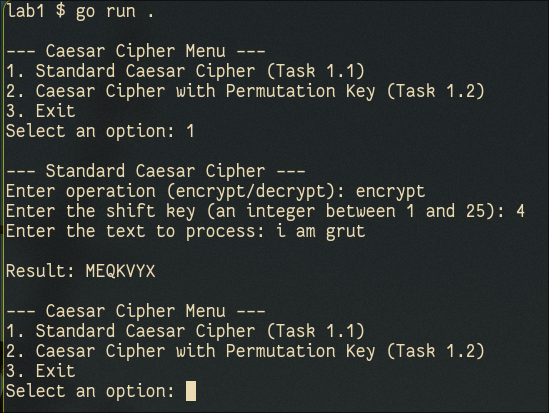
\includegraphics[width=.9\linewidth]{./results/caesar_enc.png}
\caption{\label{fig:org06489fa}Standard Caesar Encryption}
\end{figure}

\begin{figure}[htbp]
\centering
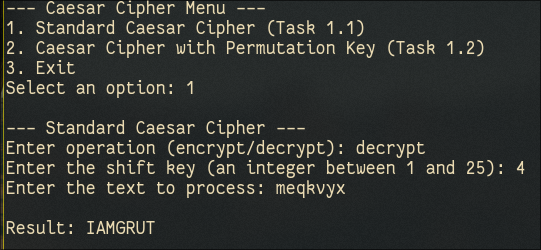
\includegraphics[width=.9\linewidth]{./results/caesar_dec.png}
\caption{\label{fig:org4093e58}Standard Caesar Decryption}
\end{figure}
\end{enumerate}
\subsection{Task 1.2: Permutation Caesar Cipher (Two Keys)}
\label{sec:orgdfb6dd2}
\subsubsection{Overview}
\label{sec:org2e85329}
This extended cipher uses both a shift key \(k_{1}\) (integer) and a permutation key \(k_{2}\) (keyword string) to create a custom alphabet ordering before applying the Caesar shift.
\subsubsection{Implementation}
\label{sec:org03fcd7c}
The \texttt{getPermutationKey} function validates that \(k_{2}\):
\begin{itemize}
\item Contains only alphabetic characters
\item Has a minimum length of 7 characters
\end{itemize}
\begin{Code}
\begin{Verbatim}
\color{EFD}\EFk{func} \EFf{getPermutationKey}(\EFv{reader} *\EFt{bufio.Reader}) \EFt{string} \{
        \EFk{for} \{
                fmt.\EFf{Print}(\EFs{"Enter the permutation keyword (at least 7 letters long, "} +
                          \EFs{"no numbers/symbols): "})
                \EFv{key}, \EFv{\_} := reader.\EFf{ReadString}(\EFs{'\char92{}n'})
                key = strings.\EFf{TrimSpace}(key)

                \EFv{cleanKey} := \EFf{sanitizeText}(key)

                \EFk{if} \EFb{len}(cleanKey) < 7 \{
                        fmt.\EFf{Println}(\EFs{"Invalid keyword. It must contain at least 7 letters."})
                        \EFk{continue}
                \}
                \EFk{if} \EFb{len}(cleanKey) != \EFb{len}(key) \{
                        fmt.\EFf{Println}(\EFs{"Invalid keyword. It must contain only letters "} +
                                    \EFs{"('A'-'Z', 'a'-'z')."})
                        \EFk{continue}
                \}
                \EFk{return} key
        \}
\}
\end{Verbatim}
\end{Code}
The \texttt{generatePermutedAlphabet} function sanitizes and uppercases the keyword \(k_{2}\), appends unique letters from \(k_{2}\) to the new alphabet in order of first appearance, appends remaining standard alphabet letters (A-Z) not in \(k_{2}\) in their natural order.
\begin{Code}
\begin{Verbatim}
\color{EFD}\EFk{func} \EFf{generatePermutedAlphabet}(\EFv{keyword} \EFt{string}) \EFt{string} \{
        \EFk{var} \EFv{builder} \EFt{strings.Builder}
        \EFv{seen} := \EFb{make}(\EFk{map}[\EFt{rune}]\EFt{bool})

        \EFcd{// }\EFc{Add unique characters from the keyword first}
        \EFk{for} \EFv{\_}, \EFv{char} := \EFk{range} strings.\EFf{ToUpper}(keyword) \{
                \EFk{if} \EFnc{!}seen[char] \{
                        builder.\EFf{WriteRune}(char)
                        seen[char] = \EFo{true}
                \}
        \}

        \EFcd{// }\EFc{Add the rest of the alphabet}
        \EFk{for} \EFv{\_}, \EFv{char} := \EFk{range} alphabet \{
                \EFk{if} \EFnc{!}seen[char] \{
                        builder.\EFf{WriteRune}(char)
                \}
        \}

        \EFk{return} builder.\EFf{String}()
\}
\end{Verbatim}
\end{Code}

The results are shown in Figures \ref{fig:orgcec9131}, \ref{fig:orgf34e517}
\begin{figure}[htbp]
\centering
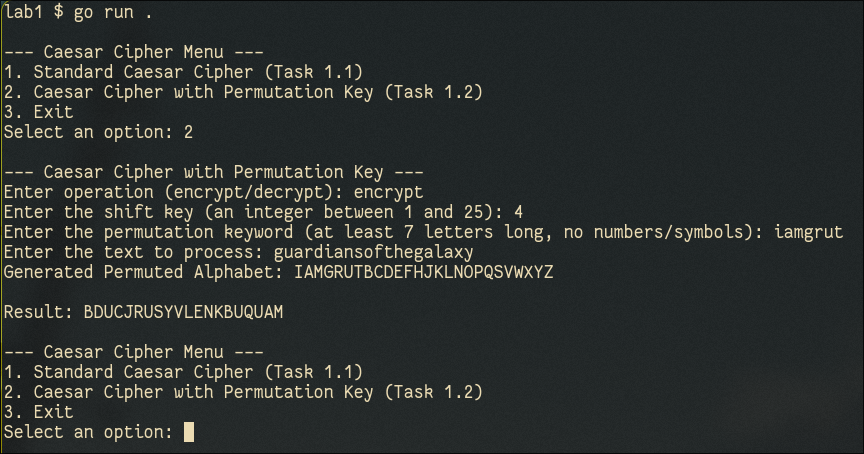
\includegraphics[width=.9\linewidth]{./results/extended_caesar_enc.png}
\caption{\label{fig:orgcec9131}Extended Caesar Encryption}
\end{figure}

\begin{figure}[htbp]
\centering
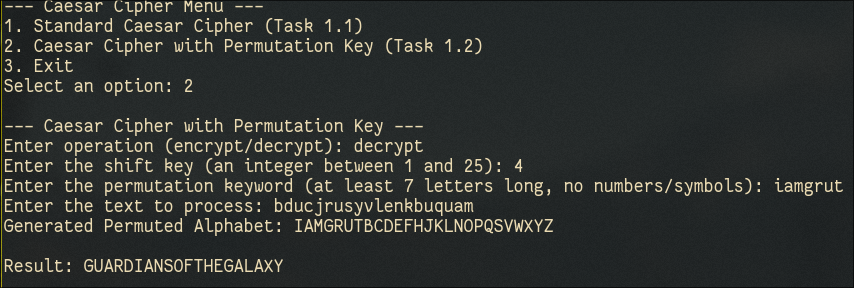
\includegraphics[width=.9\linewidth]{./results/extended_caesar_dec.png}
\caption{\label{fig:orgf34e517}Extended Caesar Decryption}
\end{figure}
\subsection{Task 1.3: Cipher Verification (Exchange and Decrypt)}
\label{sec:org426ea34}
\subsubsection{Objective}
\label{sec:org5043ff3}
This task verifies the practical application of the Permutation Caesar Cipher through a peer exchange, where two students encrypt messages and exchange them for decryption verification.
\subsubsection{Exchange Results}
\label{sec:orgf91239b}
\textbf{My Encryption:}
\begin{itemize}
\item Original message: \texttt{TESTMESSAGE}
\item Shift key (\(k_{1}\)): \texttt{7}
\item Permutation key (\(k_{2}\)): \texttt{SECURITY}
\item Generated permuted alphabet: \texttt{SECURITYABDFGHJKLMNOPQVWXZ}
\item Resulting ciphertext: \texttt{HAYHXAYYKOA}
\end{itemize}
\textbf{Partner's Encryption:}
\begin{itemize}
\item Received ciphertext: \texttt{XZHHIXJZB}
\item Provided shift key (\(k_{1}\)): \texttt{4}
\item Provided permutation key (\(k_{2}\)): \texttt{MOLDOVA}
\item Generated permuted alphabet: \texttt{MOLDVABCEFGHIJKNPQRSTUWXYZ}
\item Decrypted message: \texttt{SUCCESSFUL}
\end{itemize}
Both encryption and decryption processes were successful. The decrypted message matched the partner's original plaintext, confirming correct implementation of the permutation Caesar cipher algorithm.
\section{Testing and Results}
\label{sec:orgf8d9fcf}
The implementation has been thoroughly tested with automated unit tests. The test results are shown in Figure \ref{fig:org89413a5}.
\begin{figure}[htbp]
\centering
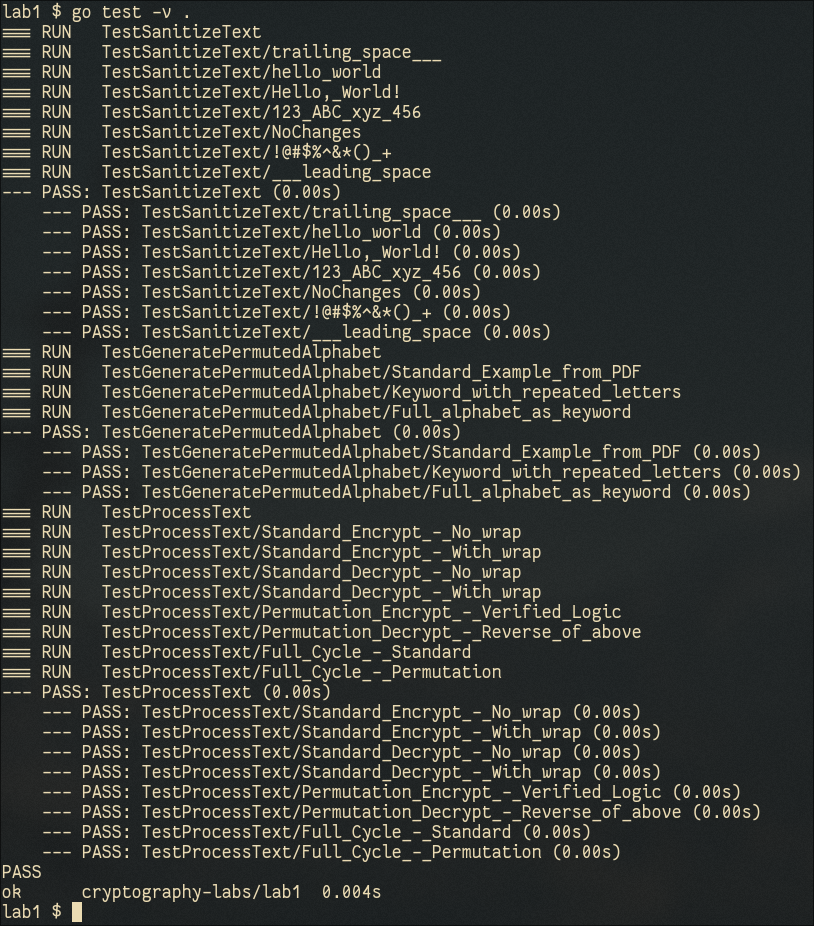
\includegraphics[width=.9\linewidth]{./results/tests.png}
\caption{\label{fig:org89413a5}Test results}
\end{figure}
\subsection{Test Coverage}
\label{sec:org4cac38e}
The following test cases have been implemented:
\subsubsection{TestSanitizeText}
\label{sec:org08114ad}
Validates text sanitization functionality with various input patterns:
\begin{itemize}
\item Trailing spaces: \texttt{"hello world "} to \texttt{HELLOWORLD}
\item Standard text: \texttt{"hello\_world"} to \texttt{HELLOWORLD}
\item Greeting variations: \texttt{"Hello, World!"} to \texttt{HELLOWORLD}
\item Alphanumeric combinations: \texttt{"123 ABC xyz 456"} to \texttt{ABCXYZ}
\item Special character handling: \texttt{"!@\#\$\%\textasciicircum{}\&*()\_+"} to \texttt{""}
\item Leading space removal: \texttt{" test"} to \texttt{TEST}
\end{itemize}
\subsubsection{TestGeneratePermutedAlphabet}
\label{sec:org0ebb39a}
Tests alphabet permutation generation:
\begin{itemize}
\item Standard example from specification: \texttt{"cryptography"} to \texttt{CRYPTOGAHBDEFIJKLMNQSUVWXZ}
\item Keywords with repeated letters: \texttt{"ABRACADABRA"} to \texttt{ABRCDEFGHIJKLMNOPQSTUVWXYZ}
\item Full alphabet as keyword input
\end{itemize}
\subsubsection{TestProcessText}
\label{sec:org8aa3858}
Verifies encryption/decryption operations:
\begin{itemize}
\item Standard encryption with wrapping (e.g., \texttt{XYZ} with \(k=5\) → \texttt{CDE})
\item Standard encryption without wrapping (e.g., \texttt{ABC} with \(k=3\) → \texttt{DEF})
\item Standard decryption with wrapping (e.g., \texttt{ABC} with \(k=3\) → \texttt{XYZ})
\item Standard decryption without wrapping
\item Permutation-based encryption with verified logic
\item Permutation-based decryption (reverse operation)
\item Full cycle tests (encrypt then decrypt) for both standard and permutation methods
\end{itemize}
\subsection{Security Analysis}
\label{sec:org980a81c}
\textbf{Standard Caesar Cipher:}
Has a keyspace of 25 possible keys.
Easily broken by exhaustive key search (brute force).
\textbf{Permutation Caesar Cipher:}
Keyspace is \(26! \times 25\). Exhaustive key search becomes computationally infeasible, but it is vulnerable to frequency analysis attacks, and remains a monoalphabetic substitution cipher
(each plaintext letter always maps to the same ciphertext letter).
\section{Conclusions}
\label{sec:org08b8186}
This laboratory work successfully implemented the Caesar Cipher and its permutation-enhanced extension. The use of a permutation keyword significantly complicates an exhaustive key search compared to the standard version, although the cipher remains vulnerable to frequency analysis. All requirements regarding text sanitization (uppercase, no non-letters) and key validation (\(k_{1}\in[1,25], len(k_{2})\ge7\)) were met in the implementation.
\end{document}
